%=======================+=========================
%================  Simulation  ================
%=================================================
\section[Monte Carlo]{Monte Carlo simulation \label{sec:simulation}}
The detailed simulation of events in the Hall-D beam line and GlueX detector is performed with a Geant-based simulation.The package was originally developed within the GEANT3 framework~\cite{Brun:1987ma} and recently migrated to the GEANT4 framework~\cite{Agostinelli:2002hh,Allison:2016lfl}. The simulation framework uses the same geometry definitions and magnetic field maps as used in reconstruction and is able to simulate the primary photon beam from the bremsstrahlung radiator through the GlueX detector to the photon beam dump, as well as doing event simulations of photoproduction events in the GlueX detector itself. The simulation broadly follows the diagram as shown in Fig.~\ref{fig:MC-data-flow}. Events of interest are generated using either a predefined or user-supplied event generator. The events are read in by the Geant-based Hall-D Monte Carlo, which obtains the appropriate geometry and magnetic field information from the geometry and calibration data bases. The resulting events are then processed by a digitization package. This package obtains run-dependent information from both the calibration and run-conditions data bases and background events from a file. The simulated events have appropriate inefficiencies applied, and then together with the background events, are digitized to look like raw data from the experiment. The resulting events are then processed with same reconstruction software as used for the real events and the output is saved to a REST file. These files are then made available for physics analysis.
\begin{figure}[h!]\centering
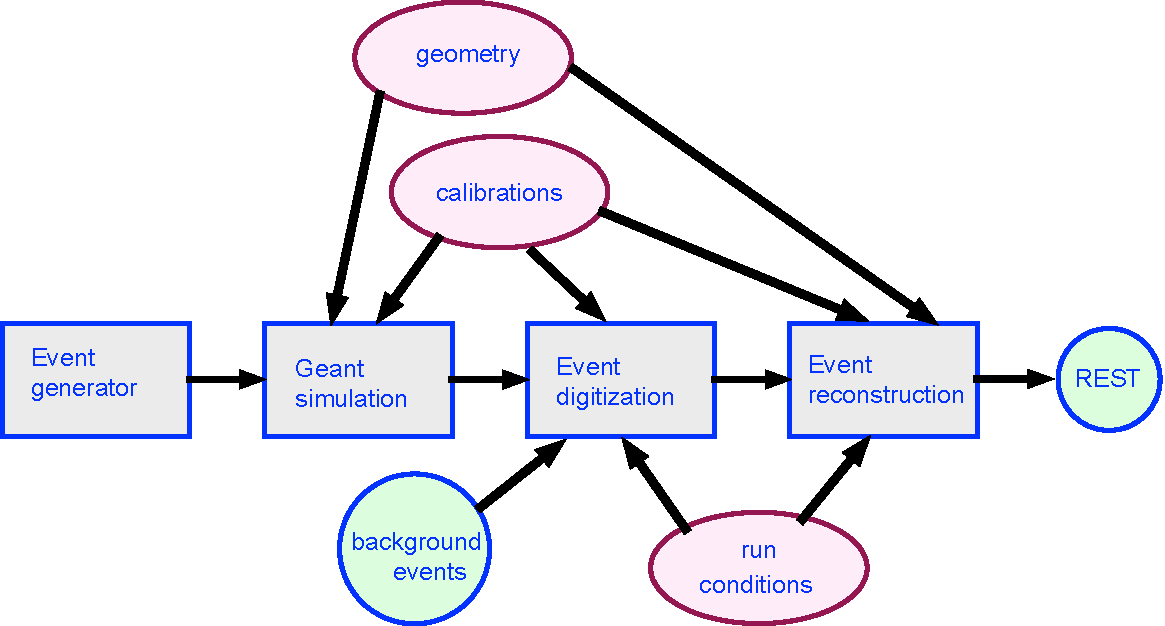
\includegraphics[width=0.85\textwidth]{figures/MC-data-flow.pdf}
\caption[]{\label{fig:MC-data-flow}The data flow from event generator through physics analysis files for Monte Carlo events.}
\end{figure}

\subsection{Event generators \label{sec:generators}}
Simulation starts with the generation of events, which can be specific particles or reactions, or a background generator. A common tool set has been developed to minimize redundancy in code. These tools include standard methods to generate the distributions of primary photon beam energies and polarization.

One of the first generators has been used to simulate the entire photoproduction cross section and is used to study backgrounds to physics reactions as well as develop analysis tools for extracting signals. This is based on Pythia~\cite{Sjostrand:2006za}, but includes additions that describe the low-energy photoproduction cross sections. 


\subsection{HDGeant \label{sec:hdgeant}}

\subsubsection[Material thickness]{\label{sec:materialscan}Geometry definitions}


\subsection[mcsmear]{Detector Response}
\subsubsection{Signal digitization}
\subsubsection{Run-dependent effects}
\subsubsection{Background Events}

\subsection{Job submission \label{sec:jobsubmission}}
